% Dokumentklassen sættes til memoir.
% Manual: http://ctan.org/tex-archive/macros/latex/contrib/memoir/memman.pdf
\documentclass[a4paper,11pt,twoside,openright,article]{memoir}
\setlrmarginsandblock{*}{2.5cm}{0.75} % højre og venstre 
\setulmarginsandblock{3cm}{*}{1.2} % top og bund 
\checkandfixthelayout[nearest] % specifikt valg af højde algoritme
 
% Danske udtryk (fx figur og tabel) samt dansk orddeling og fonte med
% danske tegn. Hvis LaTeX brokker sig over æ, ø og å skal du udskifte
% "utf8" med "latin1" eller "applemac". 
\usepackage[utf8]{inputenc}
\usepackage[danish]{babel}
\usepackage[T1]{fontenc}
\usepackage{mflogo}

%sexy pdf'er
%\usepackage[export]{adjustbox}
\usepackage{pdfpages}
\usepackage{pdflscape}

%Kompakte lister
\usepackage{paralist}
 
% Matematisk udtryk, fede symboler, theoremer og fancy ting (fx kædebrøker)
\usepackage{amsmath,amssymb}
\usepackage{bm}
\usepackage{amsthm}
\usepackage{mathtools}
\parindent=0pt 

% Fancy ting med enheder og datatabeller. Læs manualen til pakken
% Manual: http://www.ctan.org/tex-archive/macros/latex/contrib/siunitx/siunitx.pdf
\usepackage{siunitx}
 
%Fancy headers, 
%Manual: https://www.sharelatex.com/learn/Headers_and_footers
\let\footruleskip\undefined
\usepackage{fancyhdr}
\pagestyle{fancy}

 
% Indsættelse af grafik. og man kan rotere tekst in line
\usepackage{graphicx} 
\usepackage{fix-cm} 
\usepackage{soul}
\sodef\an{}{0.13em}{0em}{0em} \sodef\ann{}{0.13em}{0.5em}{0em}
 
%Fancy tabeller.
%\usepackage[table]{xcolor}
\usepackage{multirow}
\usepackage{rotating} %sidewaystables!
\usepackage{longtable} %tables spanning multible pages.
\usepackage{tablefootnote} %for at indstætte fornoter i tabeller.
\usepackage{hhline} %Fixer farvede felter
\usepackage{ltxtable} %Longtabular X
\usepackage{tabularx} %Med dynamisk bredte

%URL fodnoter
\usepackage{url}

% Reaktionsskemaer. Læs manualen for at se eksempler.
% Manual: http://www.ctan.org/tex-archive/macros/latex/contrib/mhchem/mhchem.pdf
\usepackage[version=3]{mhchem}

%Lav chapter clickable og fjern border
\usepackage{hyperref}
\hypersetup{
    colorlinks,
    citecolor=black,
    filecolor=black,
    linkcolor=black,
    urlcolor=black
}

%Table of contents settings
\setsecnumdepth{subsection} % organisational level that receives a numbers
\settocdepth{subsection}   % print table of  for level 3

%Til programkode
\usepackage{listings}
\usepackage{color}

\definecolor{dkgreen}{rgb}{0,0.6,0}
\definecolor{gray}{rgb}{0.5,0.5,0.5}
\definecolor{mauve}{rgb}{0.58,0,0.82}
 
\lstset{ 
  language=C++,                % the language of the code
  basicstyle=\footnotesize,           % the size of the fonts that are used for the code
  numbers=left,                   % where to put the line-numbers
  numberstyle=\tiny\color{gray},  % the style that is used for the line-numbers
  stepnumber=1,                   % the step between two line-numbers. If it's 1, each line 
                                  % will be numbered
  numbersep=5pt,                  % how far the line-numbers are from the code
  backgroundcolor=\color{white},      % choose the background color. You must add \usepackage{color}
  showspaces=false,               % show spaces adding particular underscores
  showstringspaces=false,         % underline spaces within strings
  showtabs=false,                 % show tabs within strings adding particular underscores
  frame=single,                   % adds a frame around the code
  rulecolor=\color{black},        % if not set, the frame-color may be changed on line-breaks within not-black text (e.g. commens (green here))
  tabsize=2,                      % sets default tabsize to 2 spaces
  captionpos=b,                   % sets the caption-position to bottom
  breaklines=true,                % sets automatic line breaking
  breakatwhitespace=false,        % sets if automatic breaks should only happen at whitespace
  title=\lstname,                   % show the filename of files included with \lstinputlisting;
                                  % also try caption instead of title
  keywordstyle=\color{blue},          % keyword style
  commentstyle=\color{dkgreen},       % comment style
  stringstyle=\color{mauve},         % string literal style
  escapeinside={\%*}{*)},            % if you want to add LaTeX within your code
  morekeywords={*,...},               % if you want to add more keywords to the set
  rangeprefix=//----------,			%Used for sexy code includes
  rangesuffix=----------,			%---||---
  includerangemarker=false,			%---||---
  literate=
  {á}{{\'a}}1 {é}{{\'e}}1 {í}{{\'i}}1 {ó}{{\'o}}1 {ú}{{\'u}}1
  {Á}{{\'A}}1 {É}{{\'E}}1 {Í}{{\'I}}1 {Ó}{{\'O}}1 {Ú}{{\'U}}1
  {à}{{\`a}}1 {è}{{\`e}}1 {ì}{{\`i}}1 {ò}{{\`o}}1 {ù}{{\`u}}1
  {À}{{\`A}}1 {È}{{\'E}}1 {Ì}{{\`I}}1 {Ò}{{\`O}}1 {Ù}{{\`U}}1
  {ä}{{\"a}}1 {ë}{{\"e}}1 {ï}{{\"i}}1 {ö}{{\"o}}1 {ü}{{\"u}}1
  {Ä}{{\"A}}1 {Ë}{{\"E}}1 {Ï}{{\"I}}1 {Ö}{{\"O}}1 {Ü}{{\"U}}1
  {â}{{\^a}}1 {ê}{{\^e}}1 {î}{{\^i}}1 {ô}{{\^o}}1 {û}{{\^u}}1
  {Â}{{\^A}}1 {Ê}{{\^E}}1 {Î}{{\^I}}1 {Ô}{{\^O}}1 {Û}{{\^U}}1
  {œ}{{\oe}}1 {Œ}{{\OE}}1 {æ}{{\ae}}1 {Æ}{{\AE}}1 {ß}{{\ss}}1
  {ç}{{\c c}}1 {Ç}{{\c C}}1 {ø}{{\o}}1 {å}{{\r a}}1 {Å}{{\r A}}1
  {€}{{\EUR}}1 {£}{{\pounds}}1
}

%Til at udregne forskel mellem sider, brug \pagedifference{A}{B} mellem to labels A og B.
\usepackage{refcount}
\newcommand{\pagedifference}[2]{%
  \number\numexpr\getpagerefnumber{#2}-\getpagerefnumber{#1}\relax}
 
%Til at lave referencer med:
\usepackage{cite}

%Til at lave eksterne \ref til \labels
\usepackage{xr}

%Til at lave \Beam (DC symbol)
\usepackage{marvosym}

%Forsøg på nice lister i tabeller
\usepackage[shortlabels]{enumitem}

\newenvironment{packed_enum}{
\begin{enumerate}[1., topsep=0pt, nosep, partopsep=0pt, itemsep=0pt, parsep=0pt]
}{\end{enumerate}}

\newenvironment{packed_item}{
\begin{itemize}[•, topsep=0pt, nosep, partopsep=0pt, itemsep=0pt, parsep=0pt]
}{\end{itemize}}

%Lækker kommando til at skrive I2C flot uden at bruge \textsuperscript hver gang:
\newcommand*{\IIC}{\texorpdfstring{I\textsuperscript{2}C }{I2C }}

%Lorem ipsum
\usepackage{lipsum}


\usepackage{longtable}
\usepackage{array} % for extrarowheight

%Juicy columntypes - http://tex.stackexchange.com/questions/12703/how-to-create-fixed-width-table-columns-with-text-raggedright-centered-raggedlef
\newcolumntype{L}[1]{>{\raggedright\let\newline\\\arraybackslash\hspace{0pt}}p{#1}}
\newcolumntype{C}[1]{>{\centering\let\newline\\\arraybackslash\hspace{0pt}}p{#1}}
\newcolumntype{R}[1]{>{\raggedleft\let\newline\\\arraybackslash\hspace{0pt}}p{#1}}
\newcolumntype{Z}{>{\raggedright\arraybackslash}X}

%Dejlig kommando til at få nye kapitler på højre side
\newcommand*\cleartorightpage{%
	\clearpage
 	\checkoddpage
	\ifoddpage
  		%do nothing
	\else
		\thispagestyle{empty}
		\mbox{}
 		\clearpage
	\fi
}


%Hacky løsning til at ordne indholdsfortegnelsen.. Why memoir class.. WHY??!
\renewcommand*{\cftdotsep}{1}
\setpnumwidth{3em}
\setrmarg{4em}

%Bugfix til Longtables
\makeatletter
\def\LT@start{%
  \let\LT@start\endgraf
  \endgraf\penalty\z@\vskip\LTpre
  \dimen@\pagetotal
  \advance\dimen@ \ht\ifvoid\LT@firsthead\LT@head\else\LT@firsthead\fi
  \advance\dimen@ \dp\ifvoid\LT@firsthead\LT@head\else\LT@firsthead\fi
  \advance\dimen@ \ht\LT@foot
  \edef\restore@vbadness{\vbadness\the\vbadness\relax}% (added)
  \vbadness=\@M % (added)
  \dimen@ii\vfuzz
  \vfuzz\maxdimen
    \setbox\tw@\copy\z@
    \setbox\tw@\vsplit\tw@ to \ht\@arstrutbox
    \setbox\tw@\vbox{\unvbox\tw@}%
  \vfuzz\dimen@ii
  \restore@vbadness % (added)
  \advance\dimen@ \ht
        \ifdim\ht\@arstrutbox>\ht\tw@\@arstrutbox\else\tw@\fi
  \advance\dimen@\dp
        \ifdim\dp\@arstrutbox>\dp\tw@\@arstrutbox\else\tw@\fi
  \advance\dimen@ -\pagegoal
  \ifdim \dimen@>\z@\vfil\break\fi
      \global\@colroom\@colht
  \ifvoid\LT@foot\else
    \advance\vsize-\ht\LT@foot
    \global\advance\@colroom-\ht\LT@foot
    \dimen@\pagegoal\advance\dimen@-\ht\LT@foot\pagegoal\dimen@
    \maxdepth\z@
  \fi
  \ifvoid\LT@firsthead\copy\LT@head\else\box\LT@firsthead\fi\nobreak
  \output{\LT@output}%
}
\makeatother
\title{Rapport \\ AutoGreen \\ Gruppe 9}
\author{ 3. Semesterprojekt E3PRJ3-02 \\ Ingeniørhøjskolen, Aarhus Universitet \\ Vejleder: Tore Arne Skogberg}
\date{\today}

\fancyhf{}
\fancyhead[LO,RE]{Gruppe 9 - ''AutoGreen''}
\fancyhead[CE,CO]{Rapport}
\fancyhead[RO,LE]{IHA, AU}
\fancyfoot[CO,CE]{\nouppercase{\leftmark}}
\fancyfoot[RE,LO]{\thepage}

%Så man kan hive samtlige \labels i projektdokumentationen, alle har prefix "P-"
\externaldocument[P-]{../Projektdokumentation/projektdokumentation}

\begin{document}
\frontmatter
\maketitle

\vfill

\begin{table} [h]
	\centering
	\begin{tabular}{|l|r|l|}
	\hline 
	\textbf{Navn} & \textbf{Studienummer} & \textbf{Underskrift~~~~~~~~~~~~~~~~~~~~} \\ \hline
	Morten Hasseriis Gormsen & 201370948 & \\ && \\ \hline
	Kristian Thomsen & 201311478 & \\ && \\ \hline
	Philip Krogh-Pedersen & 201311473 & \\ && \\ \hline
	Lasse Barner Sivertsen & 201371048 & \\ && \\ \hline
	Henrik Bagger Jensen & 201304157 & \\ && \\ \hline
	David Erik Jensen & 11229 & \\ && \\ \hline
	Kasper Torp Samuelsen & 201311498 & \\ && \\ \hline
	Kristian Søgaard Sørensen & 20115255 & \\ && \\ \hline
	\end{tabular}
\end{table}

\newpage

\thispagestyle{plain}
\lipsum[1-2]
\lipsum[1-2]

\clearpage

\thispagestyle{plain}
\tableofcontents
\thispagestyle{plain}

\newpage
\setcounter{page}{1}
\mainmatter
\chapter{Indledning}
\label{ch:Indledning}

Denne rapport omhandler udvikling og realisering af en prototype til et system, der kan installeres i et drivhus. 
Systemet - AutoGreen - hjælper brugeren med at opnå og fastholde optimale forhold for planterne i drivhuset.
Systemets vigtigste funktioner er måling og regulering af temperatur, samt måling af jordfugt.
Reguleringen af temperatur sker ved hjælp af et varmelegeme, ventilatorer og åbning/lukning af et vindue. 
Ved manglende fugtighed i jorden gives brugeren besked herom. 

AutoGreen er både for den uerfarne bruger, der har brug for hjælp for at sikre sine drivhusplanters overlevelse, men det er også for den mere erfarne bruger, der ønsker optimerede forhold i sit drivhus. 
Opvarmning af drivhuset medvirker til forlængelse af vækstsæsonen og rettidig vanding af planterne er med til at sikre optimale vækstforhold. 

Controlleren og brugerfladen i AutoGreen - realiseret på et DevKit8000 - kommunikerer via UART med et PSoC 4 Pioneer Kit, der agerer \IIC master i systemet. 
Masteren kommunikerer flere \IIC slaver, der har ansvar for hhv. aktuatorer (varme, vindue og ventilation), måling af temperatur og analoge jordfugtsensorer.

\section{Læsevejledning}
Rapporten er, så vel som projektdokumentationen, opbygget kronologisk, dvs. efter samme rækkefølge som arbejdet er udført. Der er dog den undtagelse at accepttestspecifikationen er udarbejdet i umiddelbar forlængelse af kravspecifikationen, men selve testen er naturligvis først gennemført i slutningen af forløbet, hvorfor dette afsnit er behandlet i slutningen af både rapport og projektdokumentation. 

Bemærk at afsnittet \nameref{ch:arbejdsopgaver} (side \pageref{ch:arbejdsopgaver}) indeholder en oversigt over hvad de enkelte gruppemedlemmer har haft ansvar for - ikke nødvendigvis hvilke afsnit af rapporten (eller dokumentationen) de har skrevet. 

For dokumentationen gælder det, at hvert kapitel har en versionshistorik, hvor der ved hver indtastning er påført et gruppemedlems initialer. 
Dette betyder udelukkende at det pågældende gruppemedlem har 'siddet ved tasterne', og giver således ikke gruppemedlemmet nogen form for ansvar eller ejerskab af kapitlet. 

Ved første øjekast kan denne rapport synes væsentlig længere end de tilladte 30 normalsider. 
Se \cite{lib:dispRapport} for detaljeret disposition. 

\clearpage

\section{Ordforklaring}

\begin{table}[h]
\centering
\begin{tabularx}{\textwidth*9/10}{| l | Z |}
% header ------------------------
\hline
\textbf{Begreb} & \textbf{Forklaring} \\\hline
% header ------------------------
	Plantedatabase & 
	Plantedatabasen indeholder information om ideelle forhold for forskellige typer planter, som brugeren kunne tænkes at plante i sit fysiske drivhus. Informationen i plantedatabasen står til grund for udgangsparametre for nye planter i det virtuelle drivhus. Der findes en række systemplanter, som brugeren ikke kan redigere eller slette, men brugeren kan tilføje egne planter. \\\hline
	Datalog &
Systemet er udstyret med en log over de indsamlede data fra sensorer i systemet, og der måles og indskrives i loggen hvert minut. Denne er opbygget som en datastruktur, hvor hver logning indeholder information fra sensorerne samt et tidspunkt. \\\hline
	Systemlog &
Systemet er udstyret med en log over hvad systemet foretager sig. Dette kunne f.eks. være et indlæg når systemet foretager en måling, sender en e-mail og regulerer miljøet i drivhuset. \\\hline
	Virtuelt Drivhus &
Det virtuelle drivhus er systemets repræsentation af det fysiske drivhus. Brugeren kan tilføje planter fra plantedatabasen i det virtuelle drivhus, og på den måde give systemet indirekte oplysninger om ønskede parametre. Disse informationer lagres i systemets konfigurationsfil. \\\hline
	Fysisk Drivhus &
Ved det fysiske drivhus forstås det drivhus, hvori systemet er monteret. \\\hline
	Konfigurationsfil &
Dette er en klasse, der er placeret på DevKit8000, som indeholder brugerens konfigurationer om blandt andet notifikationer, e-mailadresser, antallet af fugtsensorer og deres unikke ID mm. \\\hline
	Notifikations e-mail &
Dette er en daglig e-mail, som brugeren kan vælge at få tilsendt. Den sendes klokken 12:00, og indeholder informationer om parametrene i det fysiske drivhus. \\\hline
	Advarsels e-mail &
Dette er en e-mail, som brugeren kan vælge at få tilsendt. Den sendes, hvis en parameter i det fysiske drivhus kommer uden for tolerancen af den ønskede værdi. \\\hline
\end{tabularx}
\end{table}

\clearpage
\chapter{Opgaveformulering}
\lipsum[1-6]
\chapter{Projektafgrænsning}
\label{ch:Projektafgraensning}

AutoGreen består af en strømforsyning, en række controllere (tre stk. PSoC 4 Pioneer Kits og et stk. DevKit8000), et varmelegeme (en USB strømspareskinne og en 100W 230V AC glødepære), fire 12V DC ventilatorer og en 12V steppermotor - samt tilhørende mosfet drivere. 
AutoGreen uindeholder desuden sensorer til måling af lufttemperatur, jordfugt, lysintensitet og luftfugtighed.

Selve det fysiske drivhus er således ikke en del af systemet. 
Under udviklingen af denne prototype er anvendt en model af et drivhus på ca. 33 liter, se evt. Figur \ref{P-fig:dimensioner} på side \pageref{P-fig:dimensioner} i Projektdokumenationen. 
Såfremt prototypen skal monteres i et rigtigt drivhus, skal ventilatorer og varmelegeme dimensioneres derefter.

\mbox{}

I de indledende faser af projektarbejdet - Projektformulering, Kravspecifikation, Accepttestspecifikation og Systemarkitektur - omhandler projektdokumentationen det fulde system.
Grundet tidsnød og forskellige komplikationer, er der flere dele af det samlede system, som kun er delvist eller slet ikke implementeret.
Prioriteringen af hvad der skulle skæres væk undervejs har taget udgangspunkt i MoSCoW prioriteringen, se afsnit \ref{ch:Opgaveformulering} \nameref{ch:Opgaveformulering} på side \pageref{ch:Opgaveformulering}.

Alle punkter under "Systemet skal"\ er fuldt implementeret. 

Under "Systemet bør"\ er det første punkt, vedrørende jordfugtsensorer, fuldt implementeret; øvrige punkter er kun delvist eller slet ikke implementeret.

Punkter under "Systemet kan"\ og "Systemet vil ikke i denne version"\ er ikke implementeret. 

Det er med fuldt overlæg at denne løbende prioritering har fundet sted. 
Gruppen ønskede fra starten et system med mange muligheder for udvikling og udbygning; derfor blev der fra begyndelsen beskrevet et system, som var væsentligt mere omfattende, end hvad gruppen regnede med at kunne nå at realisere.

\mbox{}

Den gennemførte acceptest (af hele det beskrevne system) giver detaljeret information om hvad der er realiseret, hvad der er delvist realiseret og hvad der ikke er realiseret, se afsnit \ref{P-ch:Accepttest} \nameref{P-ch:Accepttest} på side \pageref{P-ch:Accepttest} i projektdokumentationen. 


\clearpage
\chapter{Systembeskrivelse} \label{ch:Systembeskrivelse}

Det system, der er tænkt realiseret i dette projekt, er en skalamodel af et drivhus med steppermotor til åbning af et vindue og blæsere til udluftning samt et varmelegeme til at varme drivhuset op. 
Til at måle på drivhuset var det tiltænkt at implementere en temperatursensor, jordfugtmålere samt sensorer til måling af lysintensitet og luftfugtighed. 
De to sidstnævnte er dog ikke implementeret grundet komplikationer i implementeringsfasen.

Selve systemet styres af et DevKit8000, som brugeren af systemet kan interagere med.
På denne platform kører - samtidigt med det grafiske miljø - processer til regulering og monitorering af miljøet i drivhuset.
Der er udover dette også mulighed for at tilgå forudindstillede planter i en plantedatabase samt at tilføje og fjerne eksisterende planter i et virtuelt drivhus, som systemet anvender til at afspejle de planter, der eksisterer i det fysiske drivhus.
Al aktivitet omkring styringen af systemet logges i en systemlog.

\begin{figure}[h]
\centering
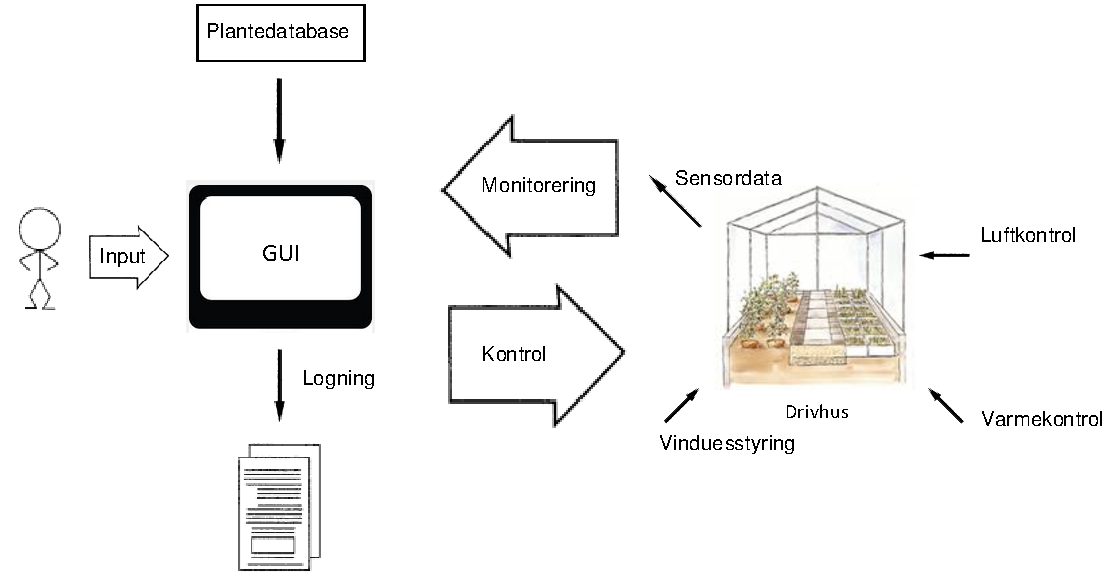
\includegraphics[width=\textwidth]{../fig/Rigt_Billede}
\caption{Rigt billede af systemet}
\label{fig:rigt_billede}
\end{figure}

Figur \ref{fig:rigt_billede} viser et rigt billede af systemet; der ses hvordan det fysiske drivhus påvirkes ved kontrol af varme og luft samt kommunikationen med GUI'en.

\clearpage

\begin{figure}[h!]
\centering
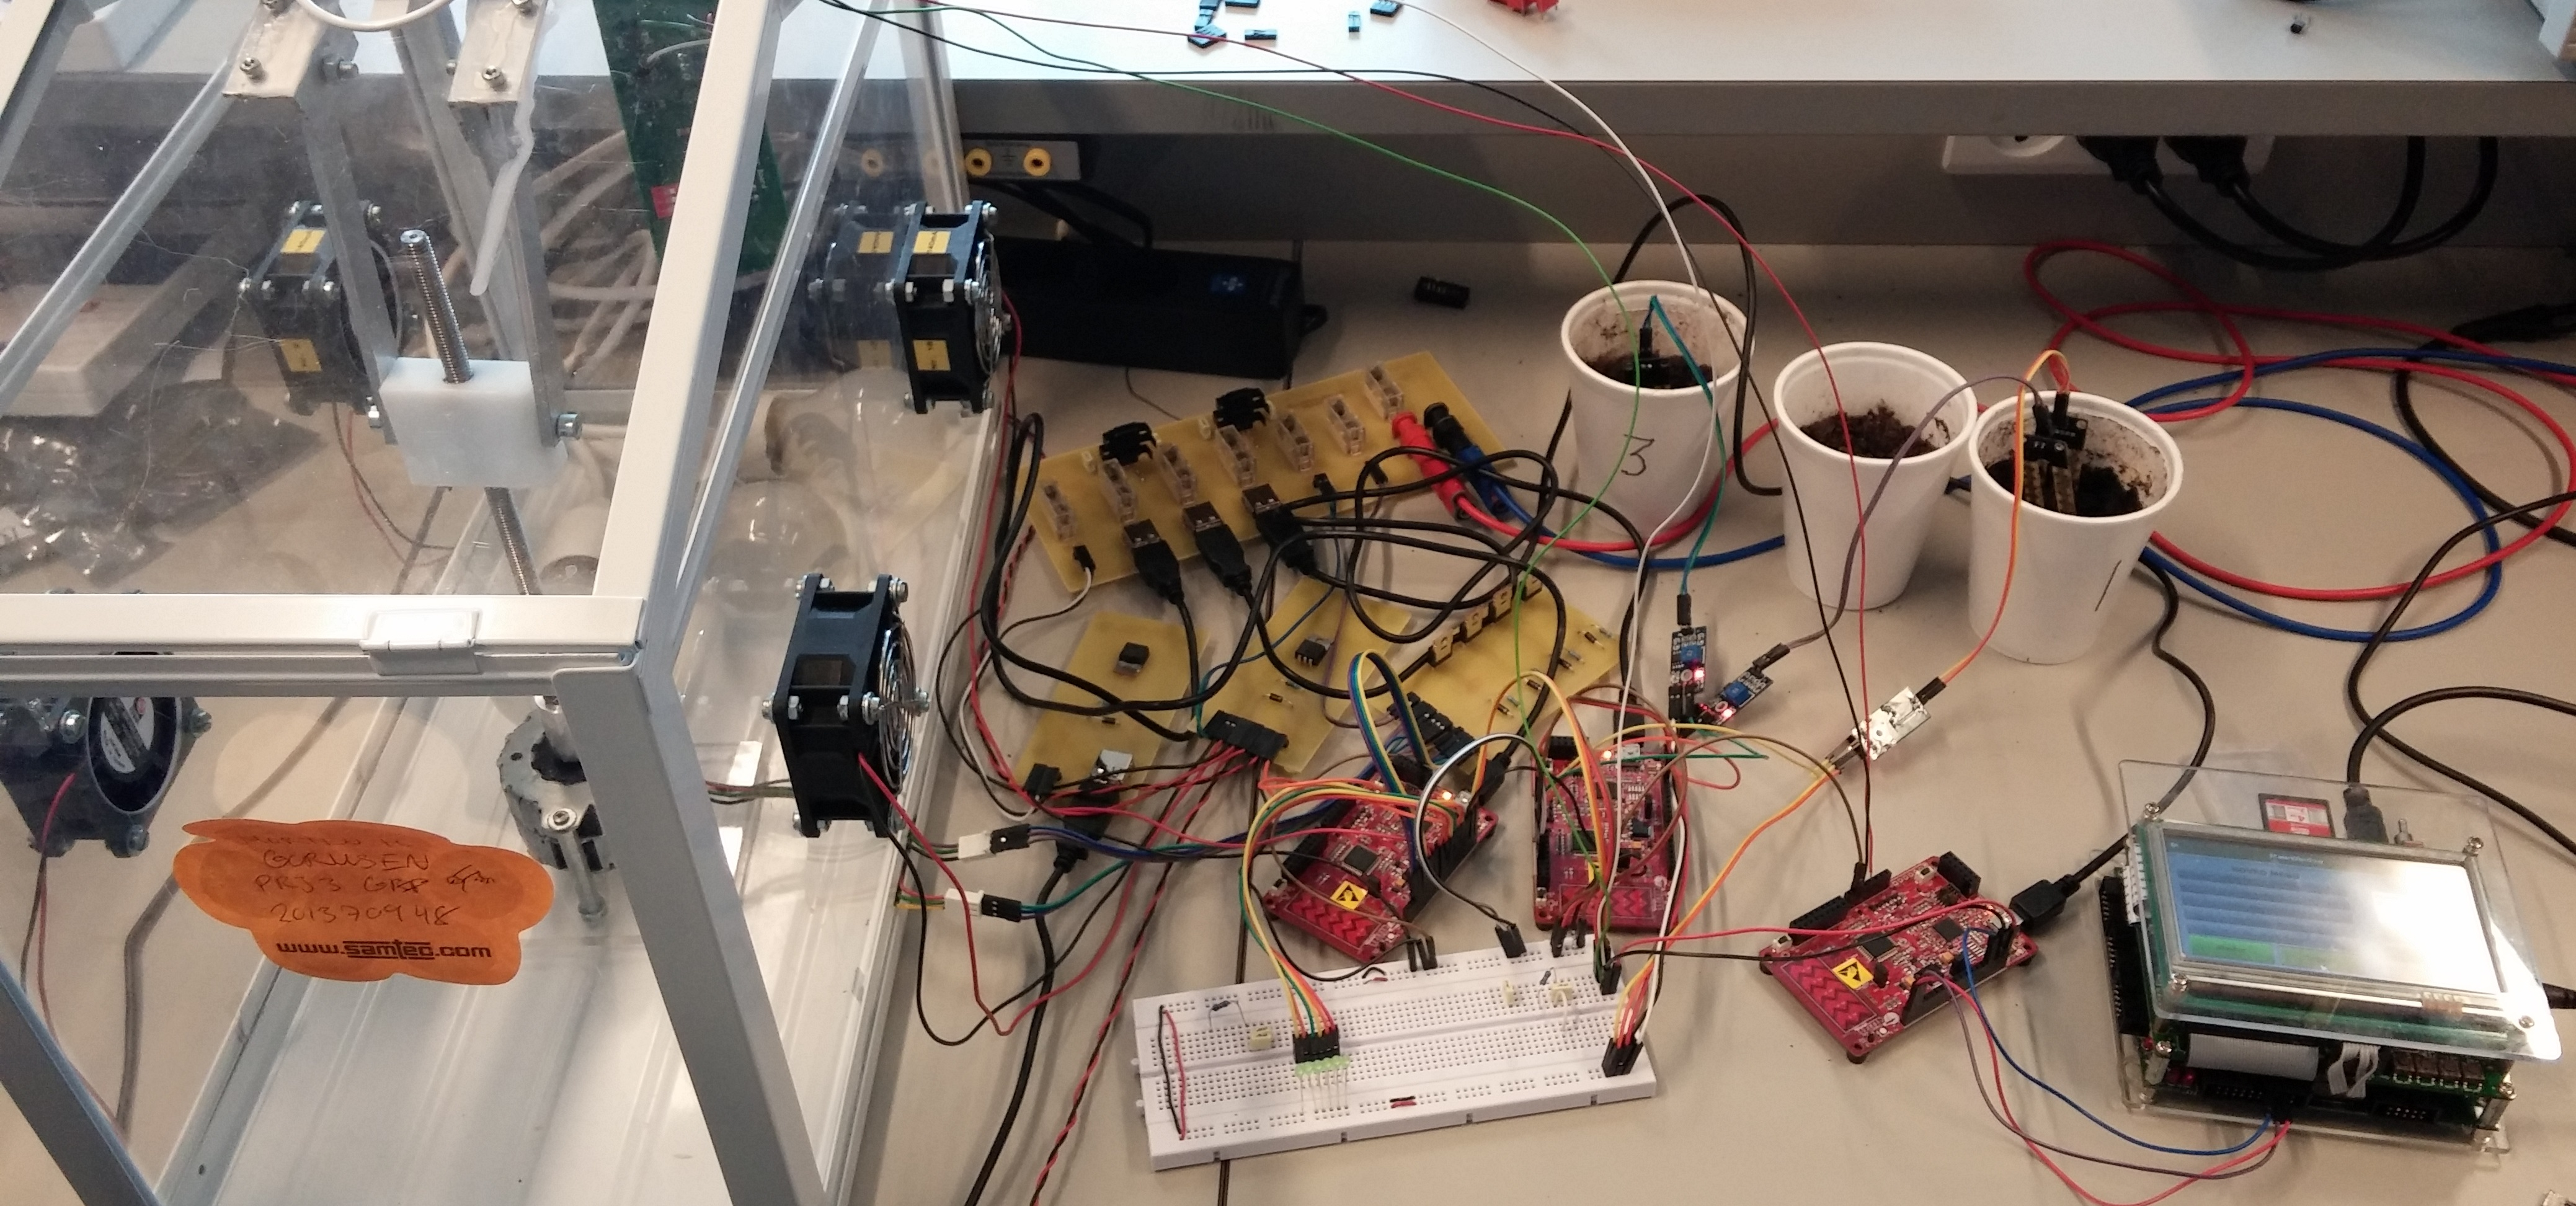
\includegraphics[width=\textwidth]{../fig/foto_system_crop}
\caption{Billede af det færdige system}
\label{fig:system_billede}
\end{figure}

På Figur \ref{fig:system_billede} ses et billede af den færdige prototype, og på Figur \ref{fig:gui_billede} ses et billede af hovedmenuen på systemets brugerflade.

\begin{figure}[h!]
\centering
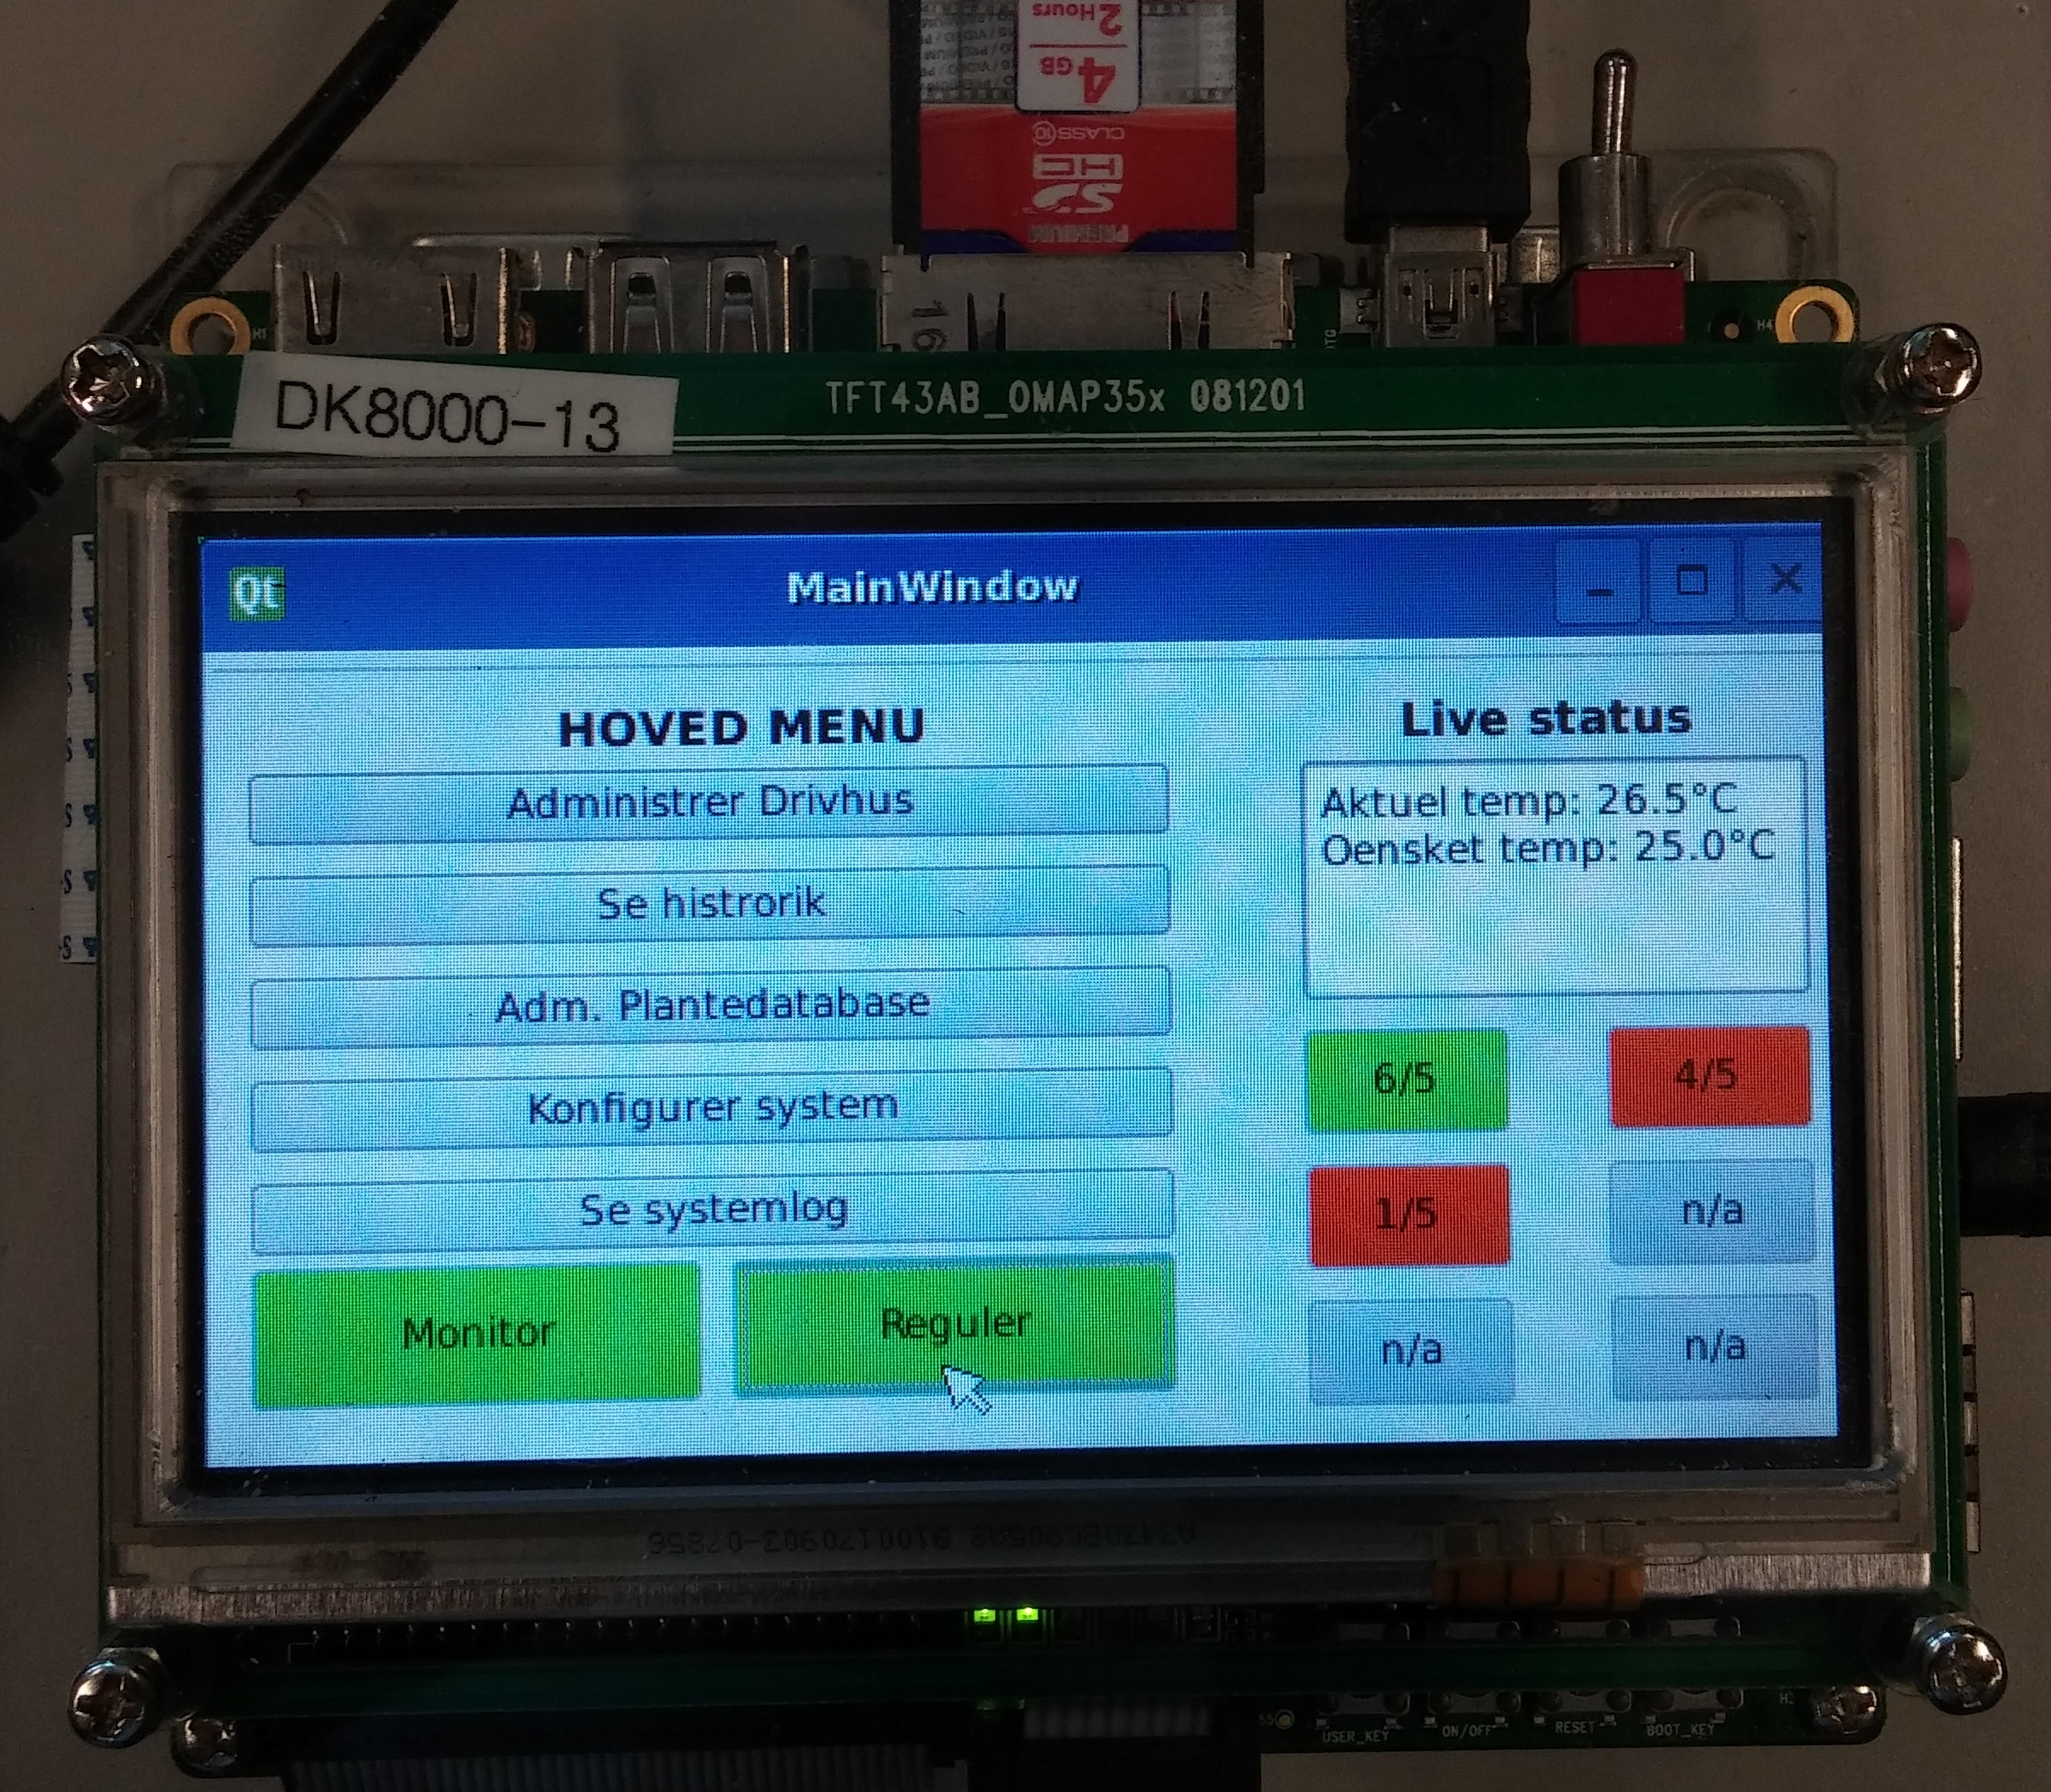
\includegraphics[width=\textwidth-5cm]{../fig/foto_gui_crop}
\caption{Billede af brugerfladen}
\label{fig:gui_billede}
\end{figure}
\chapter{Krav}
\label{ch:Krav}

I dette afsnit beskrives optillede krav for AutoGreen, som er opstillet ud fra opgaveformuleringen. 
På Figur \ref{fig:use_case_diagram} ses Use Case diagram over systemet. Dette giver et overblik over de funktionelle krav, der er formuleret i dokumentationen på side \pageref{P-ch:Kravspec}.

\begin{figure}[h]
\centering 
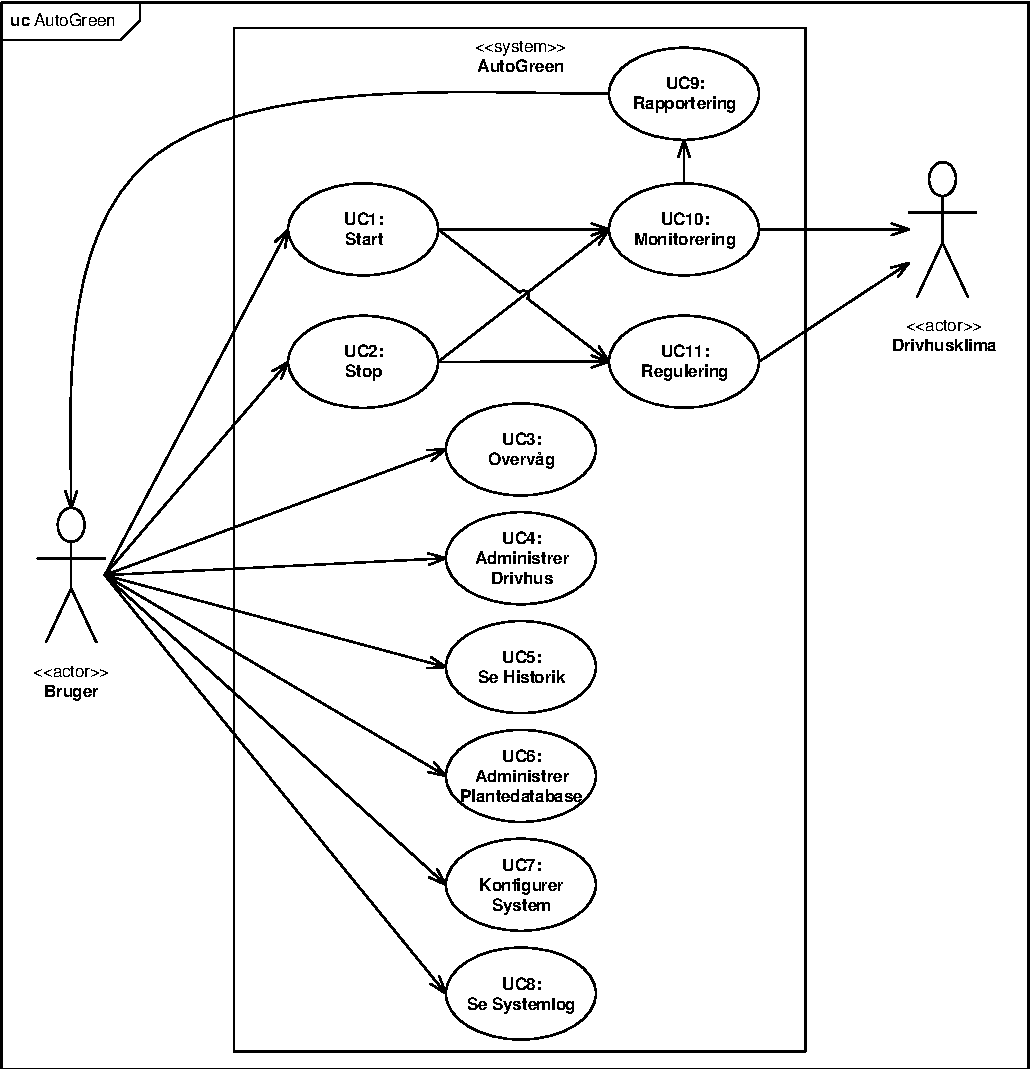
\includegraphics[width={\textwidth-1cm}, trim=0 0 0 0, clip=true] {../fig/UC_Diagram.pdf}
\caption{Use Case Diagram for AutoGreen}
\label{fig:use_case_diagram}
\end{figure}

Use Cases på billedet er kort beskrevet herunder:

\begin{itemize}

\item UC1: Start \\
Denne UC giver brugeren mulighed for at starte systemet, dvs. monitorering og regulering af drivhusklimaet.

\item UC2: Stop \\
Denne UC giver brugeren mulighed for at stoppe systemet, dvs. monitorering og regulering af
drivhusklimaet.

\item UC3: Overvåg \\
Når UC10 Monitorering er startet, vises der på brugerfladens hovedmenu alle de aktuelle måleværdier. Hvis UC11 Regulering er startet, kan værdierne for lufttemperatur og jordfugtighed være røde, hvis de ikke passer med de ønskede værdier.

\item UC4: Administrer Drivhus \\
Giver brugeren mulighed for at informere systemet om hvilke planter der er i drivhuset.

\item UC5: Se Historik \\
Giver brugeren mulighed for at se en grafisk historik over de fire målte parametre i drivhuset.

\item UC6: Administrer Plantedatabase \\
Giver brugeren mulighed for at se på planter i databasen, samt tilføje og fjerne egne planter i databasen.

\item UC7: Konfigurer System \\
Giver brugeren mulighed for at rette i systemindstillinger.

\item UC8: Se Systemlog \\
Giver brugeren mulighed for at se en liste over systemhændelser.

\item UC9: Rapportering \\
Rapporterer til brugeren ud fra de indstillinger brugeren har valgt. Dette sker ved afsendelse af e-mail til den eller de adresser som er valgt. 

\item UC10: Konfigurer System \\
Lagrer målinger af lufttemperatur, jordfugtighed, luftfugtighed og lysintensitet i en
data log.

\item UC11: Regulering \\
Regulerer temperaturen i drivhuset, vha. vinduesåbner, varmelegeme og luftcirkulation, med mindre brugeren har slået varmelegeme og/eller luftcirkulation fra.

\end{itemize}

Systemet skal have en grafisk brugerflade, der giver brugeren mulighed for at konfigurere og monitorere drivhuset. På brugerfladen skal brugeren have mulighed for at overvåge den aktuelle temperatur og bør desuden kunne se jordfugt, luftfugtighed og lysintensitet. Disse data logges og bør kunne aflæses på en graf, der viser historik for samtlige parametre. Systemet skal kunne regulere temperaturen i drivhuset på baggrund af de aktuelle parametre.\\
Baseret på brugeres præferencer kan systemet advare brugeren via e-mail, hvis systemet fejler eller klimaforholdene bliver kritiske. Til at regulere systemet skal brugeren kunne indstille systemet til at anvende varmelegeme og/eller ventilatorer til at justere klimaet. \\
AutoGreen bør have en plantedatabase, der indeholder foruddefinerede planter. Planterne kan indsættes i det virtuelle drivhus, og herefter skal systemet kunne regulere klimaet i det fysiske drivhus, så passer bedst til de(n) valgte plante(r). Brugeren skal kunne tilføje, fjerne og redigere planter, som er indsat i det virtuelle drivhus efter behov.

\clearpage
\chapter{Projektbeskrivelse}
\lipsum[1-6]

%Indsæt en masse \input her:
%\input{Projektbeskrivelse/svissen/svassen.tex}
\chapter{Konklusion}
\lipsum[1-3]
\include{Litteraturliste/Litteraturliste}

\end{document}